
\chapter{Introduction}

This introduction includes the background information, problem definition, project objective and the
research questions.

\section{Background}

Robotics in healthcare is moving from experimental pilots to practical deployment, supporting tasks such as logistics, delivery of medical supplies, and environmental assistance. These systems are intended not to replace clinical staff, but to support them by reducing repetitive physical work and enabling more time for patient care \citep{holland2021servicerobots,masala2025assistiverobotics}. As hospitals face increasing operational pressure and staff shortages, autonomous robots capable of safe navigation and interaction with the environment hold significant potential.

\begin{wrapfigure}{r}{0.36\textwidth}
    \centering
    \vspace{-8pt}
    \captionsetup{width=0.34\textwidth}
    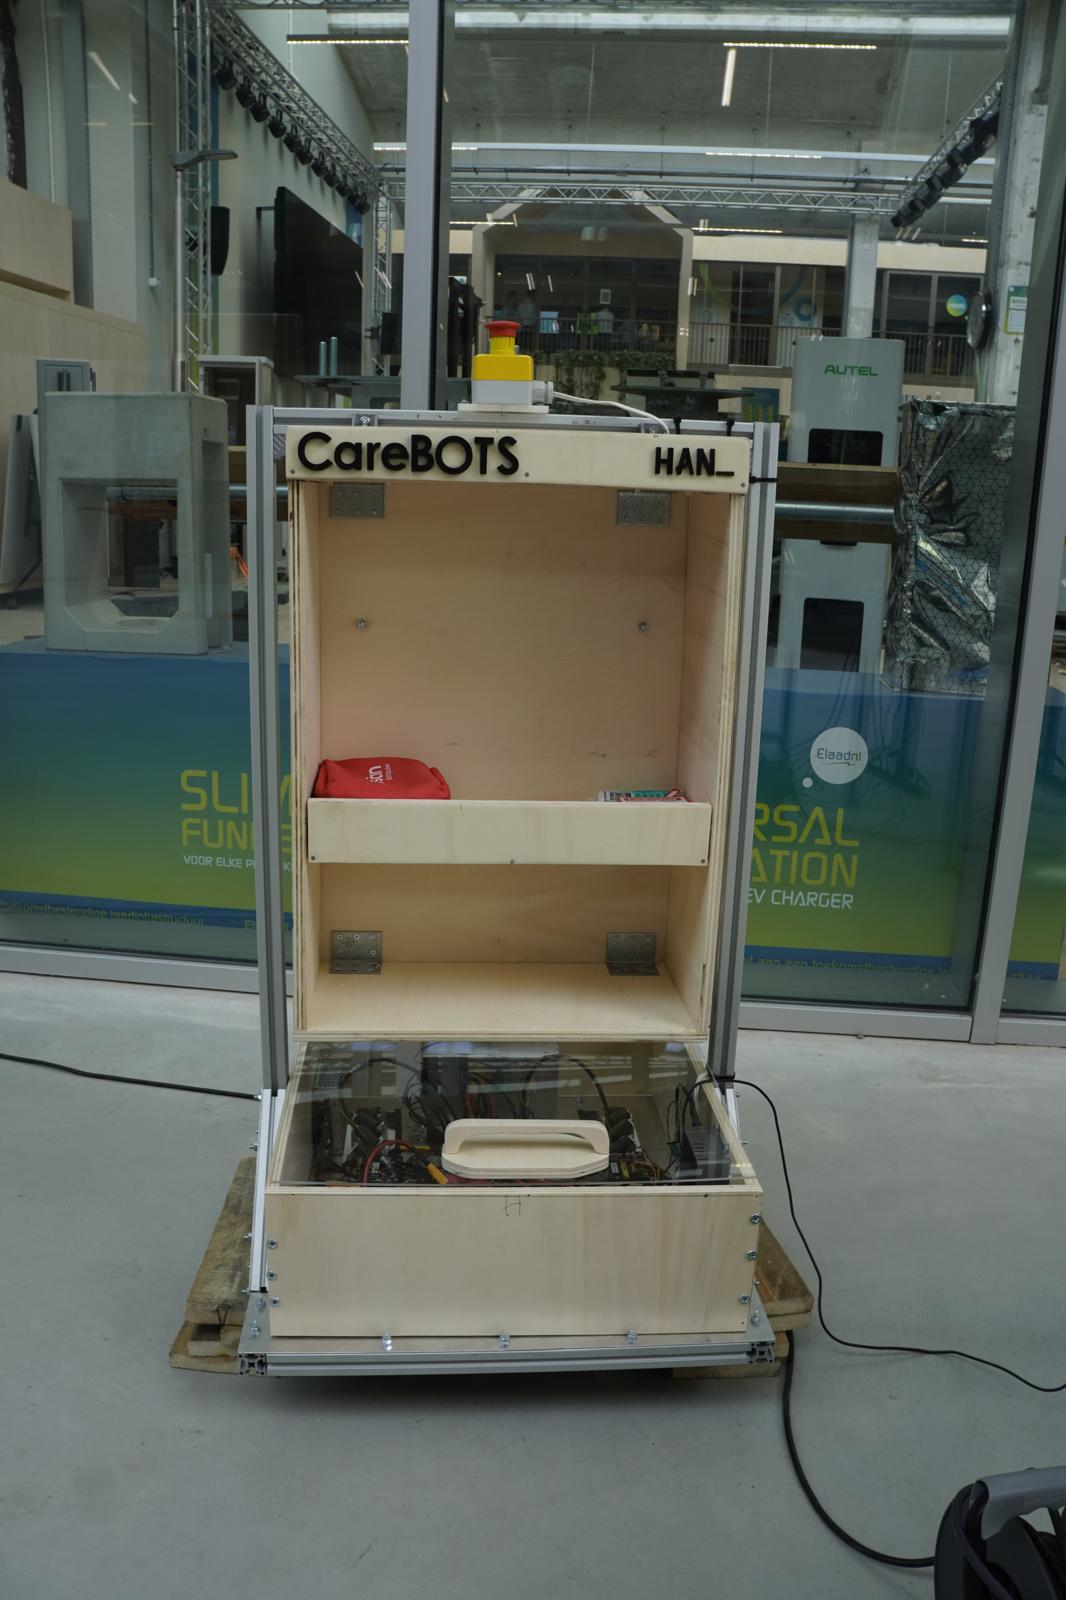
\includegraphics[width=0.45\textwidth]{figures/carebot.jpg}
    \caption{CareBot prototype at HAN Automotive Research}
    \label{fig:prototyperobot}
    \vspace{-8pt}
\end{wrapfigure}

Hospitals are typically multi-floor environments that rely on infrastructure such as elevators, automatic doors, and access-control systems. For a robot to move freely and perform tasks across different floors, it must be able to detect and interact with these human–machine interfaces, including elevator buttons and door panels. Reliable perception of such interaction elements is therefore a key capability for achieving truly autonomous navigation in hospital settings. Without this, robots remain confined to limited single-floor operation or require human assistance for vertical transport.

At \textit{HAN Automotive Research}, the CareBot platform is being developed as an educational and research project that allows students and researchers to experiment with robotic perception, planning, and control in realistic environments. While not designed to replicate the Ambyon ONE robot, the CareBot in this project will be equipped with a similar sensor stack and processing unit, enabling realistic simulation of Ambyon’s operational conditions. The Ambyon ONE itself is a service robot currently under development by \textit{Ambyon}, a Dutch startup focused on robotics for healthcare and logistics applications.

The CareBot system uses an \gls{rgbd} camera and \gls{jetson} computing module to enable on-device perception suitable for real-time operation in clinical environments. A key research challenge is enabling the robot to accurately detect and classify interaction points such as elevator buttons, access readers, and door panels under varying lighting, reflections, occlusions, and diverse panel designs - while maintaining efficient performance within embedded hardware constraints.

This project contributes to that research direction by designing and evaluating a scalable computer-vision workflow for interaction-point detection on embedded systems. The work includes dataset creation, model design and optimisation, evaluation on prototype hardware, and preparation for future extensions. The resulting system will serve as a foundation for autonomous hospital mobility and support the development of assistive robotic technologies.

%---------------------------------------------------------------

\section{Problem Definition}
% The Ambyon ONE robot currently lacks a robust and efficient perception system capable of reliably detecting and localizing human-interaction elements such as elevator buttons, door panels, and access systems in hospital environments in real time on Jetson-class embedded hardware, under variable conditions and panel layouts.
The Ambyon ONE robot currently lacks a reliable computer-vision system to detect and recognize human-interaction elements (e.g., elevator and door control interfaces) in hospital environments, preventing autonomous navigation and interaction with building infrastructure.

\section{Project Objective}
% Develop and validate an efficient and scalable computer vision workflow that enables the Ambyon ONE robot to autonomously detect and classify human-interaction elements in hospital environments using embedded hardware.
Develop and validate an efficient and scalable computer-vision workflow that enables a service-robot platform to autonomously detect and classify human-interaction elements in hospital environments using embedded hardware.

\section{Research Question(s)}
\textbf{Main Research Question:} \\
How can an efficient and scalable computer-vision workflow be designed and implemented to enable a service robot to detect and interpret human-interaction elements in hospital environments using embedded hardware?

\textbf{Sub-questions:}
\begin{enumerate}
    \item What are the relevant human–interaction points in hospital environments that should be detected and classified by the computer-vision workflow?
    \item What computer-vision methods and model architectures are most suitable for detecting and classifying human-interaction elements in service-robot environments?
    \item How can a high-quality dataset be designed and constructed for achieving robust model performance?
    \item Which model-optimization techniques support real-time inference on embedded hardware while preserving detection accuracy?
    \item How can the workflow support scalable and efficient model improvements, including potential data collection and retraining during deployment?
\end{enumerate}


\section{Outline of the report}

Chapter~1 introduces the background, motivation, and objectives of the project.
Chapter~2 reviews relevant literature on interaction-point perception, instance
segmentation, and embedded computer-vision systems. Chapter~3 describes the
methodology, including dataset preparation, annotation strategy, model training,
evaluation, and deployment considerations. Chapter~4 presents the experimental
results and quantitative evaluation. Chapter~5 discusses the findings and their
implications, and Chapter~6 concludes the report and outlines future work.

